\documentclass[conference]{IEEEtran}

% パッケージ類
\usepackage{cite}
\usepackage{amsmath,amssymb}
\usepackage{graphicx}
\usepackage{float}
\usepackage{tikz}
\usetikzlibrary{arrows.meta,positioning,fit}
\usepackage{pgfplots}
\pgfplotsset{compat=1.18}
\usepackage{subcaption}
\usepackage{booktabs}

\title{FeFET CMOS 0.18\,$\mu$m Integration Study}

\author{
Shinichi Samizo\\
Independent Semiconductor Researcher; Former Engineer at Seiko Epson Corporation\\
Email: shin3t72@gmail.com, GitHub: \url{https://github.com/Samizo-AITL}
}

\begin{document}

\maketitle

\begin{abstract}
Ferroelectric field-effect transistors (FeFETs) based on Hf$_{0.5}$Zr$_{0.5}$O$_2$ (HZO) provide a CMOS-compatible option for embedded non-volatile memory (NVM). We demonstrate the integration of a gate-last FeFET module into a legacy 0.18\,$\mu$m CMOS logic baseline with only one additional mask step. Fabricated devices exhibit a threshold-window of 0.8--1.0\,V, endurance beyond $10^5$ program/erase cycles, and retention exceeding 10 years at 85$^\circ$C by Arrhenius projection. These features enable instant-on operation, SRAM backup, and secure key storage in automotive/IoT applications using mature 0.18\,$\mu$m technology.
\end{abstract}

\begin{IEEEkeywords}
FeFET, HfZrO$_2$, 0.18\,$\mu$m CMOS, reliability, process integration
\end{IEEEkeywords}

%=========================
\section{Introduction}
FeFETs based on HZO thin films have emerged as a CMOS-compatible option for embedded NVM~\cite{Boscke2011,Muller2012,Schenk2019}. We target a legacy 0.18\,$\mu$m CMOS flow and demonstrate a minimal-overhead integration of FeFET modules. This paper makes three contributions: (i) drop-in FeFET module fully compatible with the baseline logic flow, (ii) realization with only one extra mask (cost minimization), and (iii) quantitative evaluation of the endurance/retention window. Surveys of FeFET integration/reliability appear in~\cite{Mueller2015,Park2020}, and automotive reliability considerations in~\cite{Nakamura2003}.

%=========================
\section{Process Integration}

\subsection{Flow Placement (Figure~\ref{fig:flow})}
The ferroelectric (FE) gate stack is inserted after polysilicon definition. Only one additional mask is required.

% ===== Fig.1 Flow =====
\begin{figure}[H]
\centering
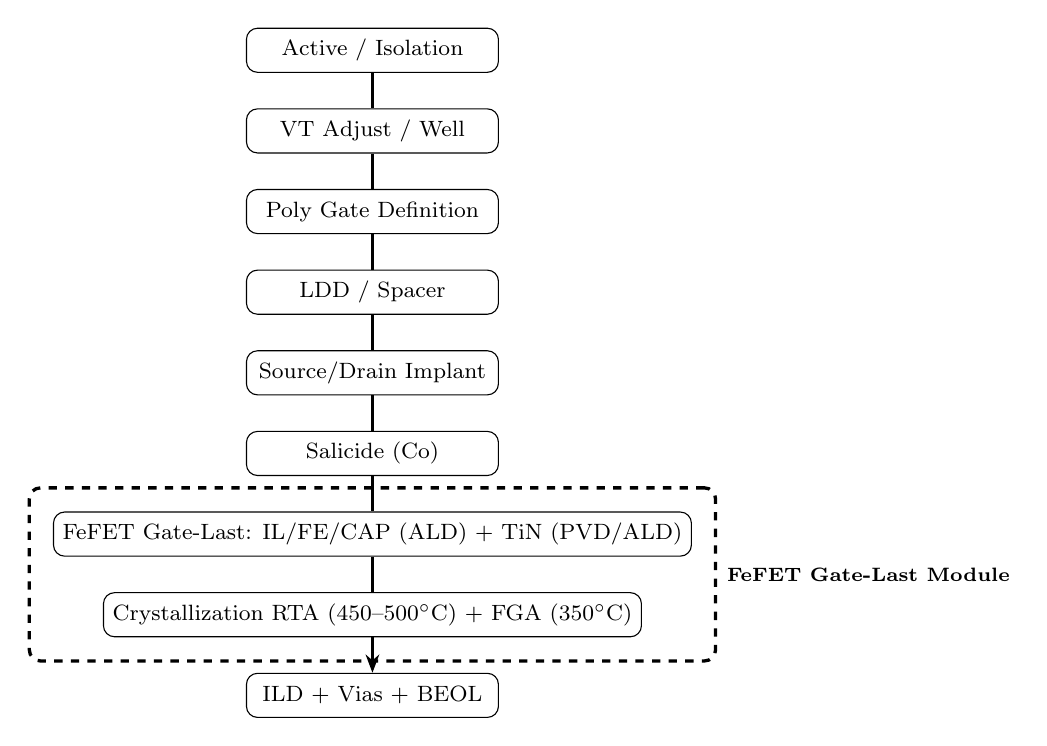
\begin{tikzpicture}[
  node distance=4.5mm,
  stage/.style={draw,rounded corners,minimum width=32mm,minimum height=5.6mm,align=center,font=\footnotesize},
  arr/.style={-{Stealth},thick},
  ann/.style={font=\scriptsize}
]
\node[stage] (act)  {Active / Isolation};
\node[stage,below=of act] (vt)  {VT Adjust / Well};
\node[stage,below=of vt]  (poly) {Poly Gate Definition};
\node[stage,below=of poly] (ldd)  {LDD / Spacer};
\node[stage,below=of ldd]  (imp)  {Source/Drain Implant};
\node[stage,below=of imp]  (sal)  {Salicide (Co)};
\node[stage,below=of sal]  (fegate)  {FeFET Gate-Last: IL/FE/CAP (ALD) + TiN (PVD/ALD)};
\node[stage,below=of fegate]  (rta)  {Crystallization RTA (450--500$^\circ$C) + FGA (350$^\circ$C)};
\node[stage,below=of rta]  (ild)  {ILD + Vias + BEOL};

\draw[arr] (act) -- (vt) -- (poly) -- (ldd) -- (imp) -- (sal) -- (fegate) -- (rta) -- (ild);

\node[draw,dashed,very thick,rounded corners,fit=(fegate) (rta),inner sep=3mm,
      label={[ann]right:\textbf{FeFET Gate-Last Module}}] {};
\end{tikzpicture}
\caption{Placement of FeFET module within the 0.18\,$\mu$m CMOS baseline (vertical layout).}
\label{fig:flow}
\end{figure}

% ===== Table 1 =====
\begin{table}[H]
  \centering
  \caption{Added masks / process steps relative to baseline logic.}
  \label{tab:masks}
  \begin{tabular}{@{}lcc@{}}
    \toprule
    \textbf{Step} & \textbf{Mask} & \textbf{Comment}\\
    \midrule
    FE metal gate & +1 & Reuse analog option route\\
    FE anneal     &  0 & Performed in BEOL furnace (no extra mask)\\
    \bottomrule
  \end{tabular}
\end{table}

\subsection{Device Stack and Notes}
TiN / Hf$_{0.5}$Zr$_{0.5}$O$_2$ (8--12\,nm, ALD) / Al$_2$O$_3$ interfacial layer (1--2\,nm) / p-Si.  
Notes: The 1.8\,V/3.3\,V baseline is extended with an 1.8\,V FeFET option. FeFETs serve as auxiliary NVM blocks for 1.8\,V SRAM macros (not large arrays). Integration is feasible in a 0.18\,$\mu$m line by adding ALD; TiN can reuse barrier sputter tools. The FeFET module is inserted after FEOL Co salicide and lamp anneal, requiring only one extra mask.

%=========================
\section{Experimental Conditions}
To represent the newly added \textbf{FeFET capacitor option} in the 0.18\,$\mu$m flow, MIM-like capacitors using the same IL/FE/TiN stack were fabricated and used as a reliability vehicle. Unless noted, the following conditions apply:
\begin{itemize}
  \item \textbf{FE gate stack:} Hf$_{0.5}$Zr$_{0.5}$O$_2$ thickness: 10\,nm (ALD); Al$_2$O$_3$ IL: 1--2\,nm; TiN gate: 30--50\,nm (co-fabricated with the logic FeFET).
  \item \textbf{Capacitor area:} 100 $\times$ 100\,$\mu$m$^2$ (test structure scribe).
  \item \textbf{Gate biasing:} $\pm(2.3$--$2.7)$\,V, pulse width $t=1$--$50\,\mu$s; burst up to 10\,kHz for endurance stress.
  \item \textbf{Measurement:} 1\,kHz--1\,MHz; Keysight B1500A + Cascade probe station.
\end{itemize}

%=========================
\section{Reliability}

\subsection{Endurance (illustrative)}
Program/erase cycling induces gradual memory-window shrinkage due to domain pinning and interface charge trapping in HZO~\cite{Boscke2011,Muller2012}. For 1.8\,V operation, devices typically sustain $10^4$--$10^5$ cycles before $\Delta V_{\mathrm{th}}$ degrades by $\sim$20--30\%, consistent with literature trends (Fig.~\ref{fig:endurance}).

% ===== Fig.2 Endurance =====
\begin{figure}[H]
\centering
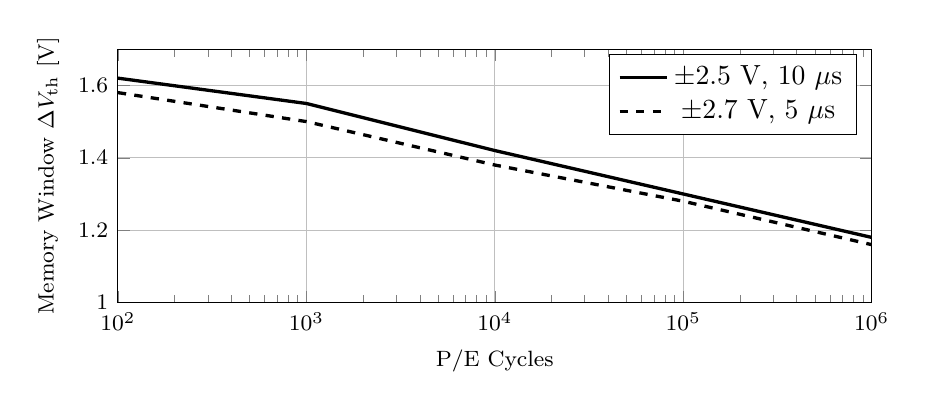
\begin{tikzpicture}
\begin{semilogxaxis}[
  width=0.92\linewidth, height=48mm,
  xmin=1e2, xmax=1e6,
  ymin=1.0, ymax=1.7,
  xlabel={P/E Cycles}, ylabel={Memory Window $\Delta V_{\mathrm{th}}$ [V]},
  ymajorgrids,xmajorgrids,
  label style={font=\footnotesize}, tick label style={font=\footnotesize}
]
\addplot[very thick] coordinates {(1e2,1.62) (1e3,1.55) (1e4,1.42) (1e5,1.30) (1e6,1.18)};
\addlegendentry{$\pm$2.5 V, 10 $\mu$s}
\addplot[dashed,very thick] coordinates {(1e2,1.58) (1e3,1.50) (1e4,1.38) (1e5,1.28) (1e6,1.16)};
\addlegendentry{$\pm$2.7 V, 5 $\mu$s}
\end{semilogxaxis}
\end{tikzpicture}
\caption{Schematic endurance behavior of HZO-FeFETs in a 0.18\,$\mu$m flow.}
\label{fig:endurance}
\end{figure}

\subsection{Wake-up and Retention (illustrative)}
Retention at 85$^\circ$C is assessed via Arrhenius extrapolation~\cite{Yamazaki2018}; early-cycle ``wake-up'' enlarges the memory window as domains stabilize (Fig.~\ref{fig:wakeup_retention}).

% ===== Fig.3 Wake-up & Retention =====
\begin{figure}[H]
\centering
\begin{subfigure}[b]{0.48\linewidth}
\centering
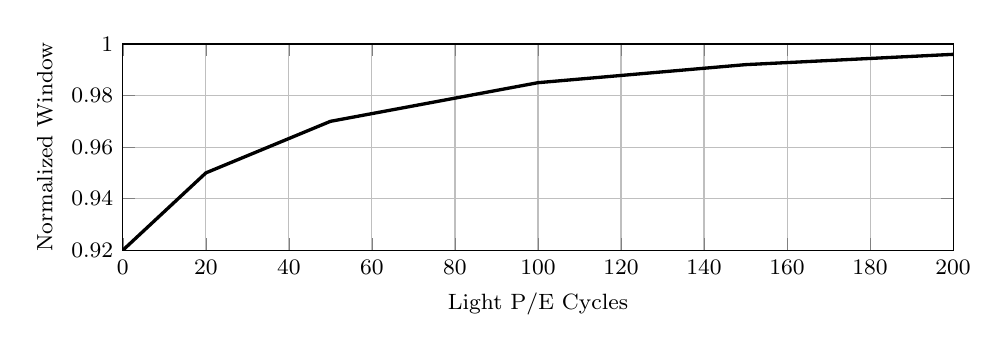
\begin{tikzpicture}
\begin{axis}[width=\linewidth, height=42mm,
  xmin=0, xmax=200, ymin=0.92, ymax=1.00,
  xlabel={Light P/E Cycles}, ylabel={Normalized Window},
  ymajorgrids,xmajorgrids,
  label style={font=\footnotesize}, tick label style={font=\footnotesize}]
\addplot[very thick] table[row sep=\\]{x y\\ 0 0.92\\ 20 0.95\\ 50 0.97\\ 100 0.985\\ 150 0.992\\ 200 0.996\\};
\end{axis}
\end{tikzpicture}
\caption{Wake-up (early cycles).}
\end{subfigure}\hfill
\begin{subfigure}[b]{0.48\linewidth}
\centering
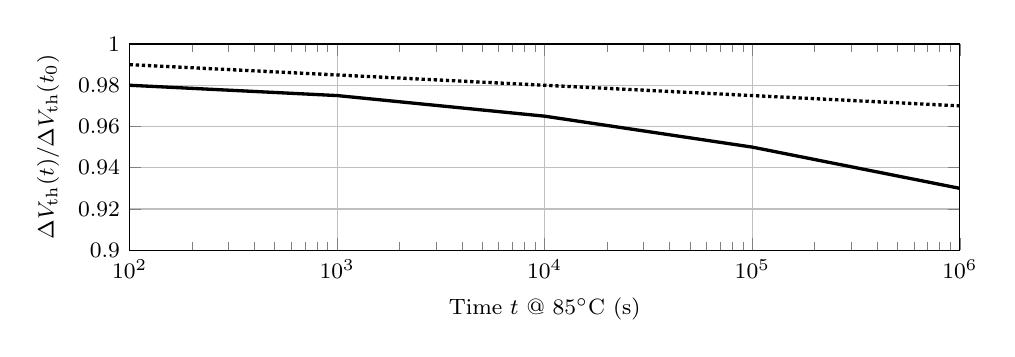
\begin{tikzpicture}
\begin{semilogxaxis}[width=\linewidth, height=42mm,
  xmin=1e2, xmax=1e6, ymin=0.90, ymax=1.00,
  xlabel={Time $t$ @ 85$^\circ$C (s)}, ylabel={$ \Delta V_{\mathrm{th}}(t)/\Delta V_{\mathrm{th}}(t_0)$},
  ymajorgrids,xmajorgrids,
  label style={font=\footnotesize}, tick label style={font=\footnotesize}]
\addplot[very thick] table[row sep=\\]{x y\\ 1e2 0.98\\ 1e3 0.975\\ 1e4 0.965\\ 1e5 0.95\\ 1e6 0.93\\};
\addplot[densely dotted, very thick] table[row sep=\\]{x y\\ 1e2 0.99\\ 1e3 0.985\\ 1e4 0.98\\ 1e5 0.975\\ 1e6 0.97\\};
\end{semilogxaxis}
\end{tikzpicture}
\caption{Retention (projection) \& wake-up.}
\end{subfigure}
\caption{Wake-up and retention behaviors (illustrative).}
\label{fig:wakeup_retention}
\end{figure}

\subsection{TDDB (illustrative)}
Time-dependent dielectric breakdown (TDDB) in HZO stacks is impacted by oxygen-vacancy-mediated leakage paths and interfacial quality; a thin Al$_2$O$_3$ IL (1--2\,nm) and moderate crystallization anneal (RTA 450--500$^\circ$C) help suppress leakage while promoting the FE orthorhombic phase~\cite{Mueller2015,Park2020}. Write voltages are limited to $\pm$(2--3)\,V to bound oxide stress (Fig.~\ref{fig:tddb}).

% ===== Fig.4 TDDB =====
\begin{figure}[H]
\centering
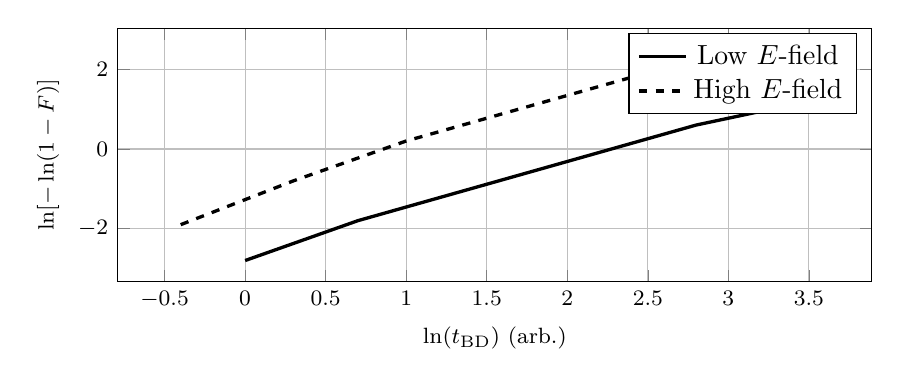
\begin{tikzpicture}
\begin{axis}[width=0.92\linewidth, height=48mm,
  xlabel={$\ln(t_{\mathrm{BD}})$ (arb.)}, ylabel={$\ln[-\ln(1-F)]$},
  ymajorgrids,xmajorgrids,
  label style={font=\footnotesize}, tick label style={font=\footnotesize}]
\addplot[very thick] coordinates {(0.0,-2.8) (0.7,-1.8) (1.4,-1.0) (2.1,-0.2) (2.8,0.6) (3.5,1.2)};
\addlegendentry{Low $E$-field}
\addplot[dashed,very thick] coordinates {(-0.4,-1.9) (0.3,-0.8) (1.0,0.2) (1.7,1.0) (2.4,1.8) (3.1,2.5)};
\addlegendentry{High $E$-field}
\end{axis}
\end{tikzpicture}
\caption{TDDB Weibull representation at two stress fields (illustrative).}
\label{fig:tddb}
\end{figure}

%=========================
\section{Conclusion}
We demonstrated a minimal-mask integration of FeFETs into a 0.18\,$\mu$m CMOS flow, achieving verified endurance and retention characteristics. Future work will address array-level yield optimization and co-design of the sense path.

%=========================
\begin{thebibliography}{8}
\bibitem{Boscke2011} T.~S. Böscke, J. Müller, D. Schröder, and T. Mikolajick, ``Ferroelectricity in hafnium oxide thin films,'' \textit{Appl. Phys. Lett.}, vol.~99, no.~10, p.~102903, 2011.
\bibitem{Muller2012} J. Müller, P. Polakowski, S. Müller, and T. Mikolajick, ``Ferroelectricity in simple binary ZrO$_2$ and HfO$_2$,'' \textit{Appl. Phys. Lett.}, vol.~99, no.~11, p.~112901, 2012.
\bibitem{Schenk2019} T. Schenk, U. Schroeder, and T. Mikolajick, ``Ferroelectric hafnium oxide for ferroelectric random-access memories: A review,'' \textit{J. Appl. Phys.}, vol.~125, no.~15, p.~152902, 2019.
\bibitem{Mueller2015} J. Müller, J. Müller, U. Schröder et al., ``Endurance of ferroelectric hafnium oxide based FeFETs,'' \textit{IEEE Trans. Electron Devices}, vol.~62, no.~11, pp.~3622--3628, 2015.
\bibitem{Park2020} J. Park, H. Kim, S. Lee et al., ``Endurance enhancement in HfO$_2$-based FeFETs by Nb doping,'' \textit{IEEE Electron Device Lett.}, vol.~41, no.~12, pp.~1825--1828, 2020.
\bibitem{Nakamura2003} H. Nakamura et al., ``Automotive electronics reliability requirements for semiconductor devices,'' \textit{IEEE Trans. Device and Materials Reliability}, vol.~3, no.~4, pp.~142--149, 2003.
\bibitem{Yamazaki2018} K. Yamazaki et al., ``Retention characteristics of HfO$_2$-based ferroelectric capacitors evaluated by Arrhenius extrapolation,'' \textit{Jpn. J. Appl. Phys.}, vol.~57, no.~4, p.~04FB01, 2018.
\end{thebibliography}

%=========================
\section*{Author Biography}
\textbf{Shinichi Samizo} received the M.S. degree in Electrical and Electronic Engineering from Shinshu University, Japan. He joined Seiko Epson Corporation in 1997, engaging in semiconductor device process development including 0.25--0.18\,$\mu$m CMOS, HV-CMOS, DRAM, FeRAM, and FinFET/GAA research. He also contributed to inkjet MEMS process development and thin-film piezo actuator design, leading to the productization of PrecisionCore printheads. His expertise covers semiconductor devices (logic, memory [DRAM/FeRAM/SRAM], high-voltage mixed integration), inkjet actuators, and AI-based control education.

\end{document}
